\documentclass[../main.tex]{subfiles}

\graphicspath{{../images/}}

\begin{document}
\pagestyle{fancy}
\chead{Module 4}
\rhead{Junseo Shin}
\lhead{CSE 4059}


\renewcommand{\thefigure}{\arabic{figure}}
\section*{Basic Matrix Multiplication}

\subsection*{Questions}

\begin{enumerate}
    \item How many floating operations are being performed in your matrix multiply
    kernel? Explain.
    
    We have 1 initialization, $2 * \texttt{numAColumns}$ from the for loop
    (multiplication and addition), and 1 assignment for the output matrix.
    Thus, for each thread, we have $2 * \texttt{numAColumns} + 2$ floating-point operations,
    and the kernel performs
    $(2 * \texttt{numAColumns} + 2) * \texttt{numCRows} * \texttt{numCColumns}$
    floating-point operations. Which is obviously $O(n^3)$.

    \item How many global memory reads are being performed by your kernel?
    Explain.

    We have 2 reads at each iteration of the for loop for the input matrices, so
    we have $2 * \texttt{numAColumns}$ global memory reads for each thread. So
    the kernel performs $2 * \texttt{numAColumns} * \texttt{numCRows} * \texttt{numCColumns}$ reads.

    \item How many global memory writes are being performed by your kernel?
    Explain.

    Since each thread writes to one element of the output matrix, we have
    $\texttt{numCRows} * \texttt{numCColumns}$ writes being performed by the kernel.

    \item Describe what possible optimizations can be implemented to your kernel
    to achieve a performance speedup.

    We can use shared memory---i.e. tiling---to reduce the number of global memory reads, and
    we could also optimize the matrix multiplication by using an algorithm that reduces the number
    of multiplications and additions needed to compute the output matrix e.g. Strassen's algorithm.
    Although one caveat with Strassen's algorithm is that it requires $2^n \times 2^n$ matrices, so
    matrices will have to be padded with zeros which could be wasteful for some matrices.

    \item Name three applications of matrix multiplication.
    
    \begin{enumerate}
        \item Image processing: 3D Gaussian splatting in computer graphics requires 
        matrix multiplication to project a `3D Guassian' onto a 2D image for real time rendering.

        \item Solving eigenvalue problems: E.g. Diagonalizing a matrix with QR decomposition requires
        iterative matrix multiplication to find the eigenvalues. Furthermore, the QR decomposition
        also requires matrix multiplication to find the orthonormal and upper triangular matrices
        e.g. using Householder reflections you need to do a bunch of matrix multiplications
        $Q = Q_1^T Q_2^T \dots$, $R = Q_2 Q_1 \dots A = Q^T A$.

        \item Image compression: JPEG compresses images using a discrete cosine transform based
        algorithm (DCT) this also translates to video and audio codec: I believe audio coding
        formats such as AAC-LP (Apple's favorite audio codec) and Opus (for the Discord users)
        use some form of the modified discrete cosine transform (MDCT) which tries to circumvent
        matrix multiplication with linear algebra tricks.
    \end{enumerate}
\end{enumerate}

\newpage
\subsection*{OUTPUT}
\begin{figure}
    [ht]
    \centering
    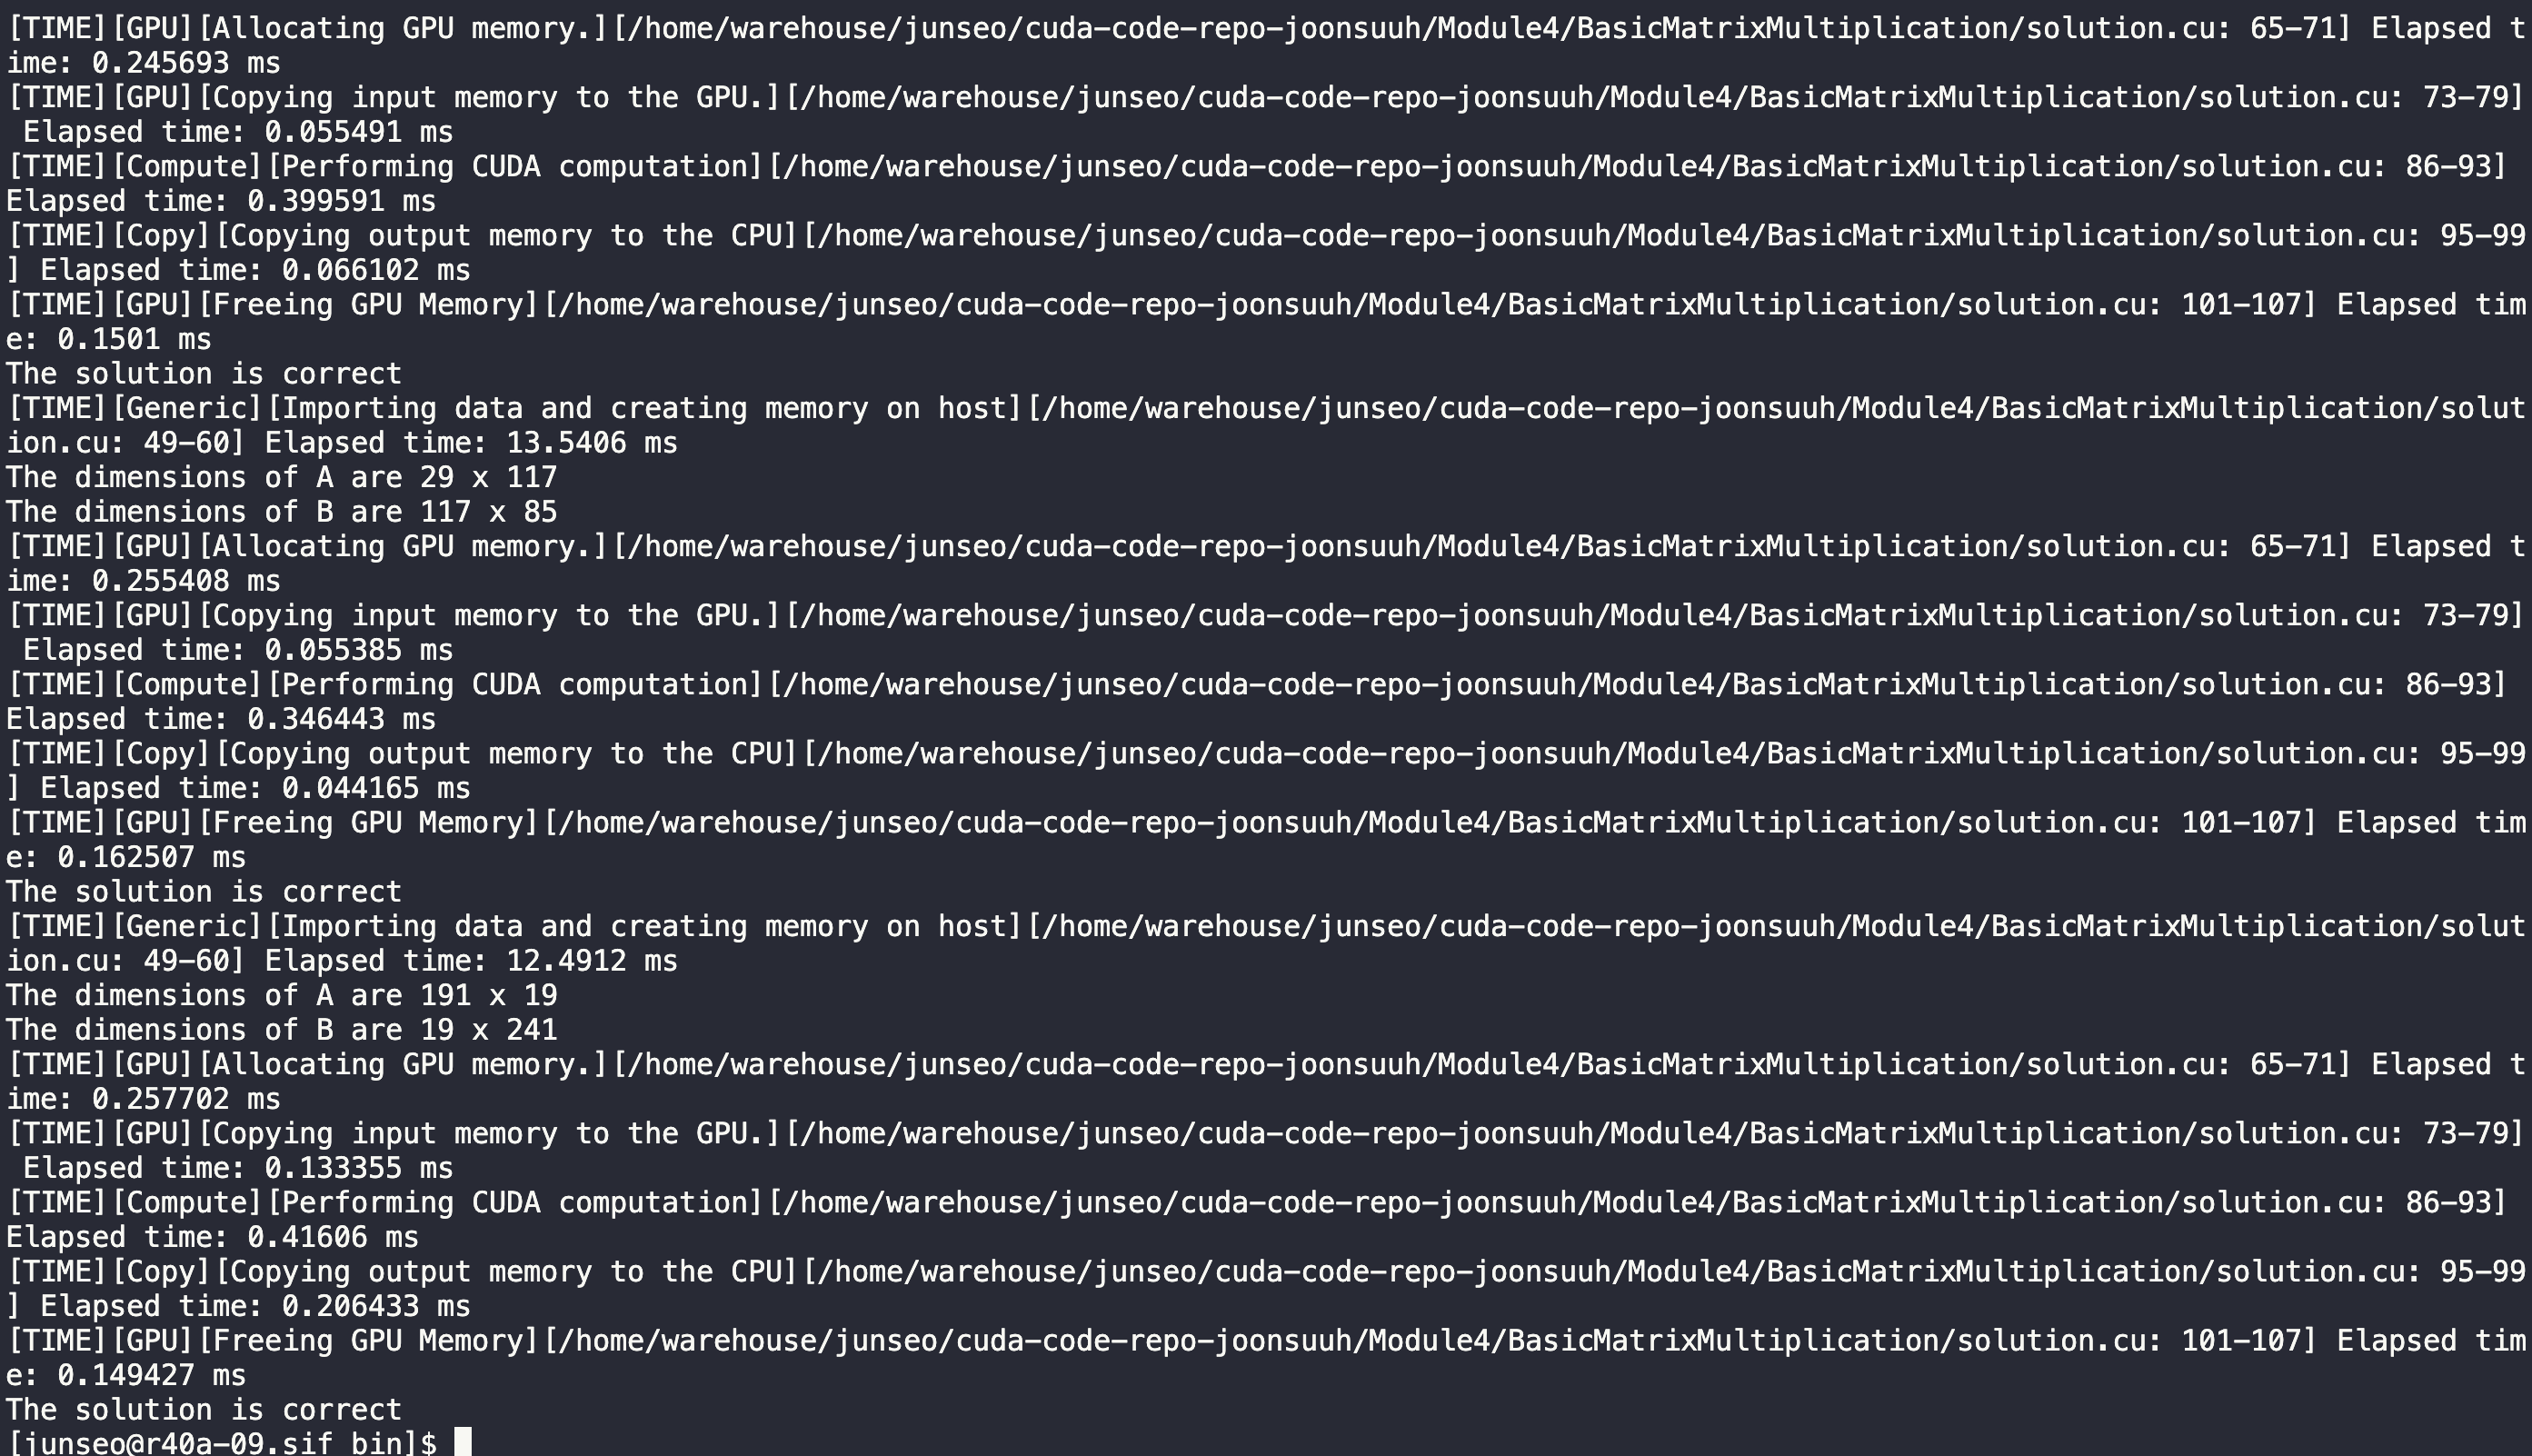
\includegraphics[width=\textwidth]{basicMatrixMult.png}
    \caption{\texttt{BasicMatrixMultiplication\_Solution} output}
\end{figure}
\end{document}